\documentclass[12pt,a4paper]{article}
\usepackage{listings}
\usepackage{hyperref}
\usepackage{graphicx}
\usepackage{float}
\usepackage{placeins}
\usepackage{subcaption}
\usepackage{amsmath}
\usepackage{cleveref}

\newcommand{\acomment}[1]{{\bf{\color{blue}{{[Aman: #1]}}}}}
\newcommand{\scomment}[1]{{\bf{\color{blue}{{[Suyash: #1]}}}}}

\hypersetup{
colorlinks=true,
allcolors=blue,
}

\usepackage{geometry}
\geometry{
a4paper,
left=20mm,
top=30mm,
}

\title{COL781: Computer Graphics\\Assignment 2}
\author{Suyash Agrawal (2015CS10262)\\Aman Agrawal (2015CS10210)}

\begin{document}
\maketitle
\section{Introduction}
    In this assignment we simulated a bowling game. There were many challenging aspects to the projects which can be roughly broken into:
    \begin{itemize}
        \item Setting up the environment including human, track, gutters, ball, pins and camera
        \item Keyframe animation of the human
        \item Controlling ball trajectory and spin
        \item Collision between ball and pin as well as between pins
    \end{itemize}
    We detail each of the above steps in the following sections.

\section{Environment}
    For setting up the environment we created the obj files for each of pin, gutter and ball. The base models for them were taken from public available models on internet, which were modified in blender (3d modelling software) and exported as obj files with their corresponding textures.
    For creating the animation, we took a base model of human from 3D animation tutorial by ThinMatrix, using which we defined our custom keyframes of bowling action and exported the whole scene in Colladae format using Blender.
    For camera, we created two modes, one which gave a free view and other which followed the ball.
    We also specified the ball velocity, ball mass, pin mass, pin fall time controllers in our code.

\section{Keyframe Animation}
    In order to do keyfrane animation, we has to create a separate model heirarchy in which we create a heirarcy of joints and associated each vertex with a set of joints. The transformation of each vertex was calculated as a weighted linear combination of transformation of the corresponding joints, and the transformation of each joint was calculated heirarchichally using the information in each keyframe.
    For interpolating the transformation between consecutive frames, we linearly interpolated the displacement vector and used quaternion interpolation for angles.
    Also, we used assimp library in order to parse the object file in colladae format.

\section{Ball trajectory}
    We modelled the trajectory of ball as a bezeir curve. We took the keypoints of the trajectory as an input in our program and correspondingly calculated the bezeir curve in which our ball will move.
    We gave forward spin to the ball in such a manner as to avoid slipping on the surface by calculating the required angular velocity of the ball in order to traverse the bezeir trajectory with a given input speed of the ball. Sideways spin was calculated in a similar manner.

\section{Collision}
    For collision handling, we internally modelled each of pin and ball as a circle projection in x-z plane. Subsequently, we wrote a procedure to check collision between two circles by checking is the distance between them is less than the sum of their radii. Then for each pair of ball and pin as well as pin and pin, we checked for a collision and if there was one, we initiated the collision effect procedure, which calculated the subsequent velocity of the colliding objects using principles of momentum conservation and elasticity. This gave a quite realistic effect of collision and pin fall.

\section{Bonus}
    We also integrated background music and collision sound in our simulation which made the whole simulation really enjoyable. We also modelled our bowler really well, which gave it a appealing and realtistic look.
    \begin{figure*}
        \begin{subfigure}[ht]{0.99\textwidth}  
            \centering 
            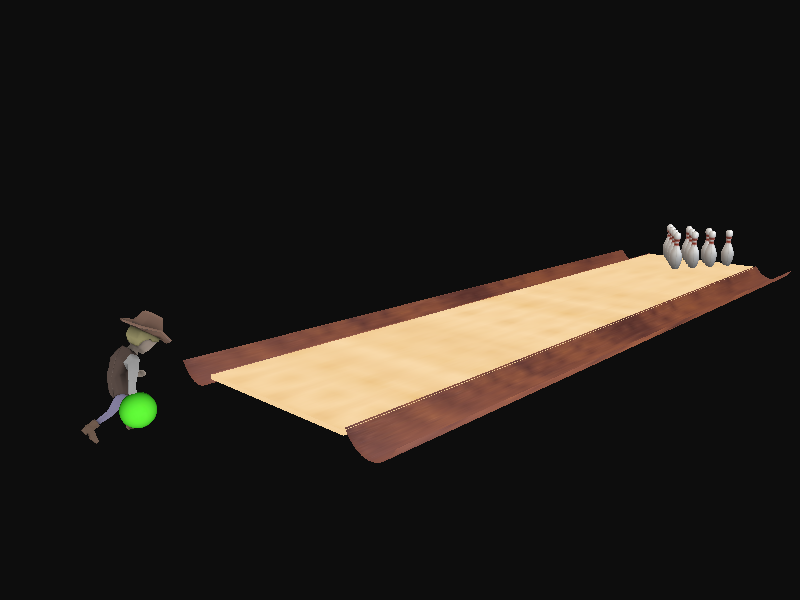
\includegraphics[width=\textwidth]{{imgs/scene}.png}
        \end{subfigure}
        \hfill
        \caption{Overview of the bowling scene}
    \end{figure*}

    \begin{figure*}
        \begin{subfigure}[ht]{0.475\textwidth}  
            \centering 
            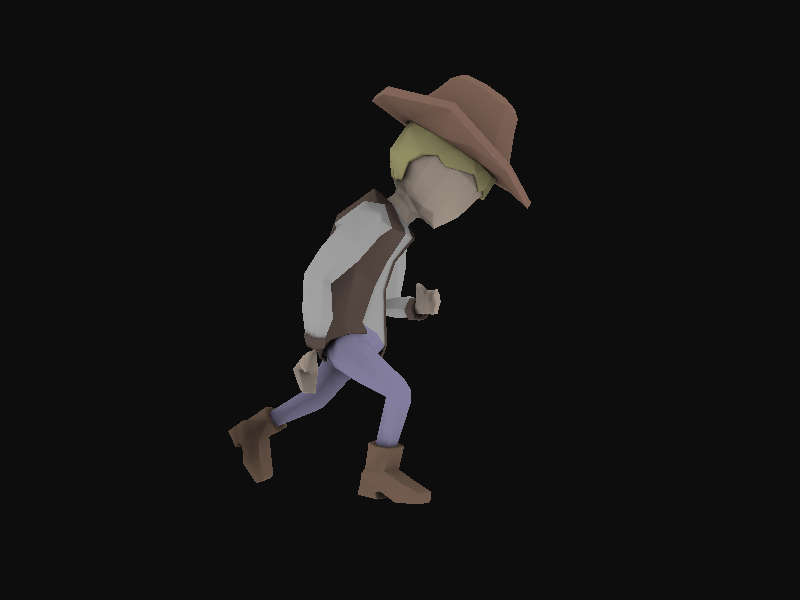
\includegraphics[width=\textwidth]{{imgs/human}.png}
            \caption{Human Model}    
        \end{subfigure}
        \hfill
        \begin{subfigure}[ht]{0.475\textwidth}   
            \centering 
            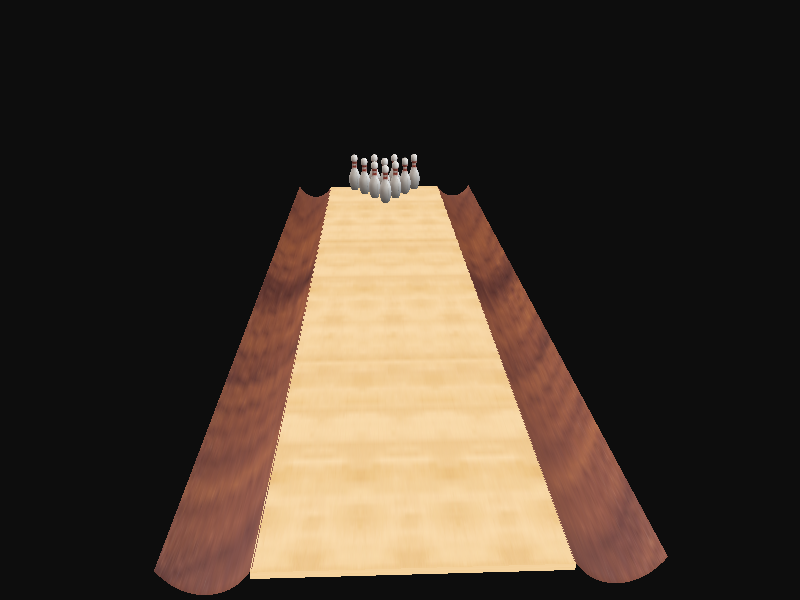
\includegraphics[width=\textwidth]{{imgs/track}.png}
            \caption{Track and pins}
        \end{subfigure}
        \vskip\baselineskip
        \begin{subfigure}[ht]{0.475\textwidth}  
            \centering 
            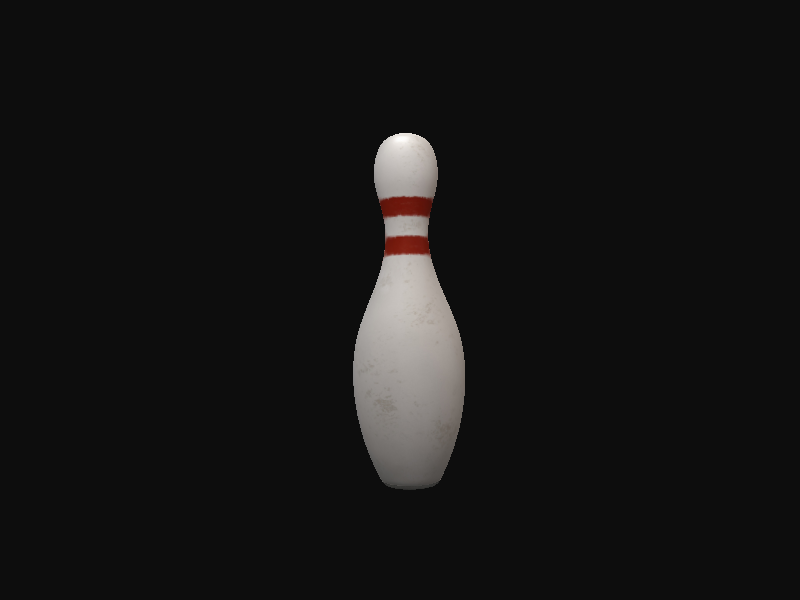
\includegraphics[width=\textwidth]{{imgs/pin}.png}
            \caption{Pin}    
        \end{subfigure}
        \hfill
        \begin{subfigure}[ht]{0.475\textwidth}   
            \centering 
            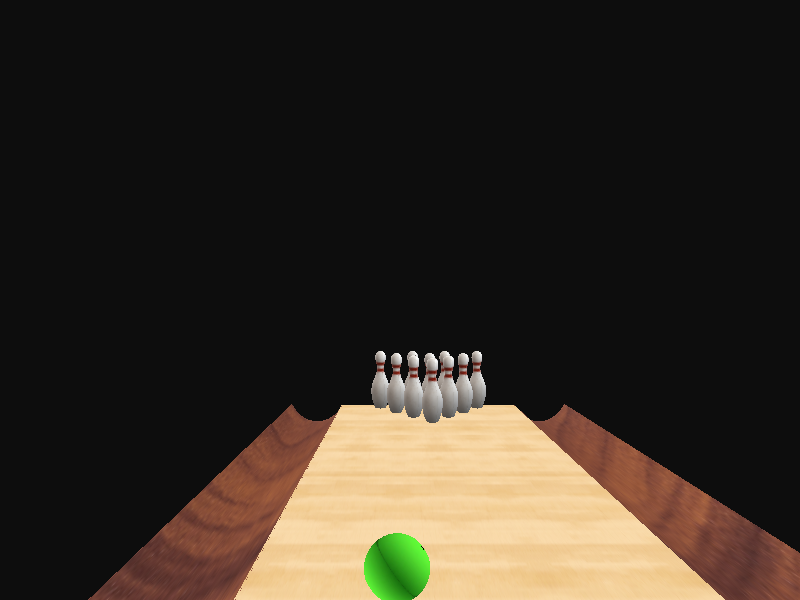
\includegraphics[width=\textwidth]{{imgs/cam_follow}.png}
            \caption{Camera Follow}
        \end{subfigure}
        \vskip\baselineskip
        \begin{subfigure}[ht]{0.475\textwidth}  
            \centering 
            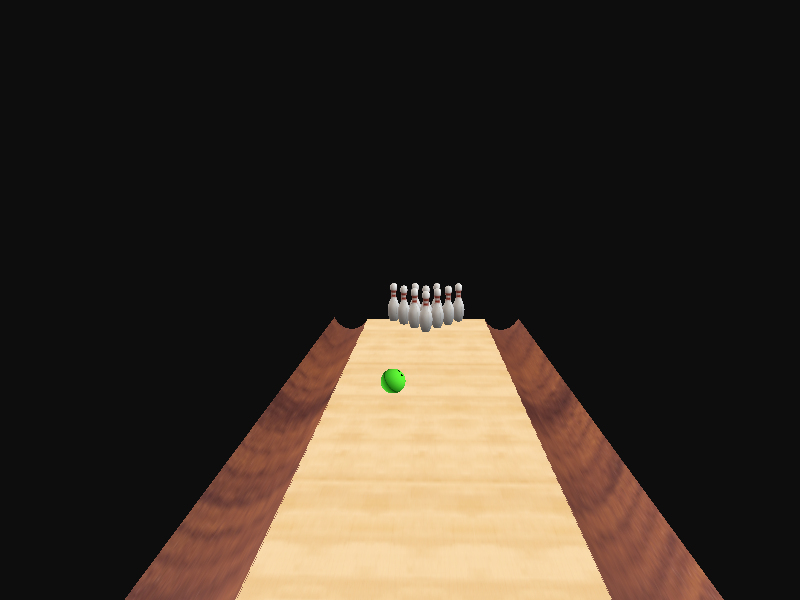
\includegraphics[width=\textwidth]{{imgs/ball_trajectory}.png}
            \caption{Ball Trajectory}    
        \end{subfigure}
        \hfill
        \begin{subfigure}[ht]{0.475\textwidth}   
            \centering 
            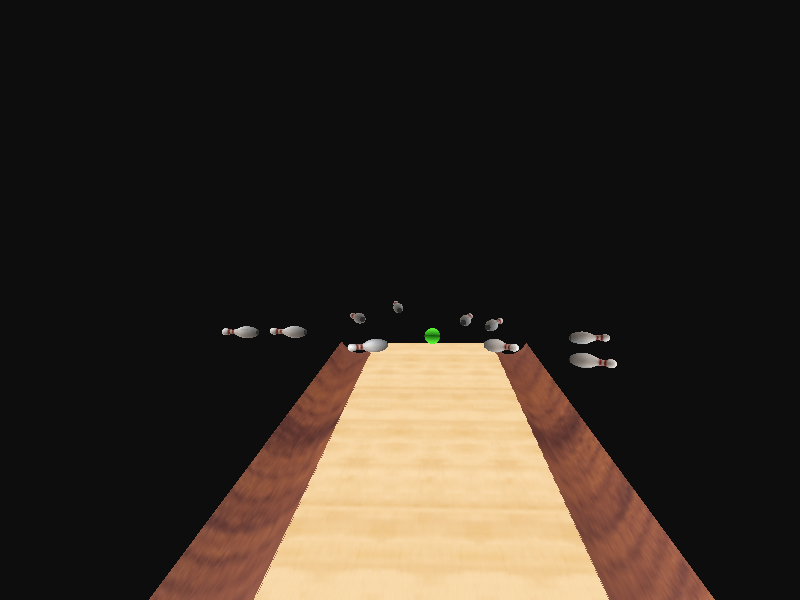
\includegraphics[width=\textwidth]{{imgs/ball_hit}.png}
            \caption{Collision}
        \end{subfigure}
        \caption{Various scenes of bowling game simulation}
    \end{figure*}

\end{document}
